\section{Physical model}\label{sec:pm}

Electrohydrodynamics involves the study of electric phenomena on fluid
flow. How fluids carrying electrical charges (electrolytes) react upon
external electrical fields or interact with charged objects are
examples of problems that arise in this field. 

As a charged object is brought into contact with an electrolyte it is,
qualitatively, easily deduced that ions with a sign of charge opposite
to that of the object will be attracted to the object and ions with
the same sign of charge will be repelled. These two distinct
categories of ions will from hereon be referred to as counter- and
co-ions respectively. In this case, for a neutral electrolyte, a
surplus of counter-ions will be present in the direct vicinity of the
object and a surplus of co-ions will be present at some other location
further from the object. The part of the net charged fluid nearest to
the charged boundary is often referred to as an electrical double
layer (EDL) \cite{dongquing-ren-book}. 

Traditionally, the physical description of EDLs and electrokinetics in
general is based on the Poisson-Boltzmann model. However the PB model
includes some crude assumptions on the system and is sometimes not an
accurate choice, see section \ref{sec:et:pb} for a brief
description. Therefore, more sophisticated modelling approaches has
been proposed e.g. in \cite{}. This paper is based on such an approach
which is described further in this section.

\subsection{Model overview}\label{sec:et:coupling}
To model the fluid motion of a charged fluid under influences of
electrostatic forces, a coupling between different models is
considered.

The electric field and potential in the system are obtained from
solving Poisson's equation (PE) for electrostatics (section
\ref{sec:et:poisson}) with a given charge density. This charge density
is obtained from a set of Nernst-Planck (NP) equations (section
\ref{sec:et:np}) by including effects on the charge distribution from
the electric field previously mentioned, diffusion and advection. One
NP equation is solved for each different ion species in the
solution. For instance in a 1:1 solution, two equations are solved one
for the positive and one for the negative ions respectively.
advective charge flux is given from the velocity field in the fluid
that is obtatined by solving the Navier-Stokes (NS) equations (section
\ref{sec:et:ns}). Forces due to present electric fields on net charged
areas of the fluid also couples the NS equations to the NP
equation. More about the force coupling is discussed in
sections. \ref{sec:et:streaming_pot} and
\ref{sec:et:electroosmosis}. The coupling between the different
equations are visualised in fig. \ref{fig:coupling}.

\nomenclature{PE, P-E}{Poisson's equation of electrostatics}
\nomenclature{NP, N-P}{Nernst-Planck equation}
\nomenclature{NS, N-S}{Navier-Stokes equations}

\begin{figure}
\begin{center}
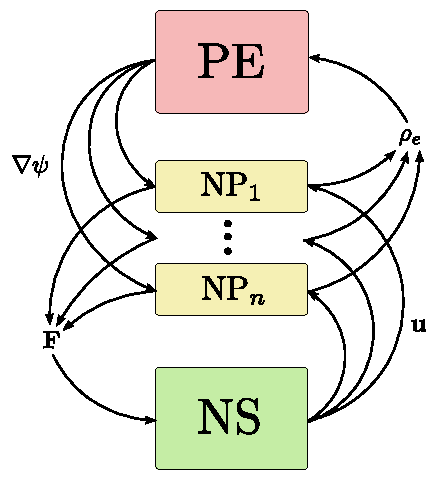
\includegraphics[width=0.5\textwidth]{fig/coupling.pdf}
\end{center}
\caption[Visualisation of the coupling between the equations
  present in the model.]{Visualisation of the coupling between the
  three equations present in the model. Poisson's equation (PE), the
  set of Nernst-Planck equations (NP$_1$ ... NP$_n$) for the different
  ion species and the Navier-Stokes equations (NS). The dependencies
  have also be marked with arrows indicating what quantities for a
  certain equation that are needed from an other.}
\label{fig:coupling}
\end{figure}

%The algorithm to solve the coupled equations is described in section
%\ref{lb:algorithm}.



\subsection{The potential - Poisson's equation}\label{sec:et:poisson}
To be able to model the flow dynamics of liquids in a channel with
present EDLs, the potential and charge distribution
in the channel must be determined. These quantities are mutually
related through Poisson's equation for electrostatics:

\begin{equation}\label{eq:pb}
\nabla^2\psirm = -\frac{\rho_e}{\epsilon_r \epsilon_0}
\end{equation}
where $\psirm$ is the electrical potential, $\rho_e$ the electrical
charge density, $\epsilon_r$ is the relative permittivity and
$\epsilon_0$ the vacuum permittivity. Under certain assumptions, the
charge density may be explicitly determined as a function of the
potential distribution, one such result is the so called
Poisson-Boltzmann equation, further discussed in section \ref{sec:et:pb}.


\subsection{The transport of charges - Nernst-Planck equation}\label{sec:et:np}
The charge concentration in an electrolyte is indeed affected by its
environment. In the model proposed here, influences from: advection of
the electrolyte, diffusion due to concentration gradients and effects
from the electric field originating from charged objects placed at the
border or in the flow is considered. Charge conservation without any
external sources of the ion density, $\C(\x, t)$, gives:

\begin{equation}\label{eq:charge_conc}
\dfrac{\partial \C}{\partial t} + \nabla \cdot \J = 0
\end{equation}
where $\mathbf{J(\mathbf{x}, \mathrm{t})}$ is the net flux induced
by the effects described above. Explicit expressions for the fluxes
due to advection and diffusion respectively are 

\begin{equation}
\J_{adv} =
\C\ubf
\end{equation}
and 
\begin{equation}
\mathbf{J}_{dif} = -D\nabla \C 
\end{equation}
where $\mathbf{u}$ is the advective velocity and $D$ is a diffusion
coefficient. The ionic flux due to the presence of an electric
potential, $\psirm(\x, t)$, is given by the Nernst equation
\cite{dongquing-ren-book}:

\begin{equation}
\J_{ele} = -\frac{zq_eD}{k_BT}\C\nabla\psirm
\end{equation}
where $z$ is the relative charge of the ion species, $q_e$ is the
fundamental charge, $k_B$ is the Boltzmann constant and $T$ is the
temperature of the fluid.

Summing up the fluxes and putting them into eq. \eqref{eq:charge_conc}
gives

\begin{equation}\label{eq:et:np}
\dfrac{\partial \C}{\partial t} = \nabla \cdot \left [
 D\nabla \C - \C\ubf + \frac{zq_eD}{k_BT}\C\nabla\psirm
\right]
\end{equation}
which is a known result often referred to as the Nernst-Planck
equation. This is the equation for the transport of \emph{one} species
of ions, if several are present one NP equation for each species needs
to be solved. The advective velocity, $\ubf$, and the potential
gradient, $\nabla \psirm$, are obtained from couplings to the
Navier-Stokes and Poisson's equation respectively. More about the
coupling between the equations is discussed in section
\ref{sec:et:coupling}.


%what we need

%nernst planck


%poisson boltzmann steady state, fix potential 

\subsection{Poisson-Boltzmann equation}\label{sec:et:pb}
Consider a system consisting of an electrolyte in contact with a
(flat) charged wall.  Under certain assumptions, it is possible to
explicitly determine the charge density in eq. \eqref{eq:et:np} as a
function of the electric potential. E.g. if there is no advection
present and if the system has reached a steady state, i.e. $\partial
\C /\partial t = 0$ and $\ubf = \mathbf{0}$ we have:

\begin{equation}\label{pb_constant_flux}
D\nabla \C + \frac{zq_eD}{k_BT}\C\nabla\psirm = \J_0
\end{equation} 
where $\J_0$ is a constant flux. Due to the steady state
assumption, what the equation above actually says is that the net flux
of charge in the system is constant. Since no charges are wanted to
flow through the wall boundary, the flux is set to zero on the wall
and since the flux is constant it will therefore be zero everywhere in
the liquid, i.e. $\J_0 = 0$.

Considering only a one-dimensional situation with a position variable
$y$ varying in a direction out from the wall into the liquid,
eq. \eqref{pb_constant_flux} reads

\begin{equation}\label{eq:pb_eq_for_C}
\frac{1}{\C} \dfrac{d \C}{d y} + \frac{zq_e}{k_BT} \dfrac{d \psirm}{d
  y} = 0.
\end{equation}

The charge density is determined by solving eq. \eqref{eq:pb_eq_for_C}
for $\C$, i.e. integrating the equation. In order to avoid introducing
additional unknown quantities, the equation is integrated to far away
from the wall where the potential from the EDL is assumed to have
decreased to zero and where the concentrations, $\C^{\infty}$, of the
electrolyte is known.

\begin{equation}
\int_y^{\infty} d\ln( \C(y')) = -\frac{z q_e}{k_BT}\int_y^{\infty}d\psirm(y')
\end{equation}
This gives an expression for $C(y)$:

\begin{equation}\label{eq:C}
\C(y) = \C^{\infty} \exp\left(-\frac{z q_e \psirm(y)}{k_BT}\right).
\end{equation}

In a general case, there may be several species of ions in the
electrolyte, the net charge density, $\rho_e$, is then given by simply
summing up the contributions from the different species:

\begin{equation}\label{eq:rho}
\rho_e = q_e\sum_i z_i \C_i.
\end{equation}

Summarising eqs. \eqref{eq:pb}, \eqref{eq:C} and \eqref{eq:rho} gives
the Poisson-Boltzmann equation in one dimension

\begin{equation}\label{eq:pb_real}
\dfrac{d^2\psirm(y)}{dy^2} = -\frac{q_e}{\epsilon_r \epsilon_0}\sum_i z_i
\C_i^{\infty} \exp\left(-\frac{z_i q_e \psirm(y)}{k_BT}\right).
\end{equation}

%% \subsubsection{The Debye–Hückel approximation}
%% Historically, the non-linear nature of eq. \eqref{eq:pb_real}
%% complicated for those wanting to solve it. This was a major difficulty
%% in the past when the computational power at hands were rather
%% limited. A linearisation is therefore sometimes done, this linear
%% version of the PB equation is often referred to as the Debye–Hückel
%% approximation. The solution of the linearisation gives, something to
%% compare with and is usually used when defining a characteristic length
%% scale of the EDL.

%% For a 1:1 electrolyte solution with an equal amount of positive and
%% negatively charged ions, eq. \eqref{eq:pb_real} reduces to

%% \begin{equation}
%% \frac{d^2\psi(x)}{dx^2} = \frac{2\C^{\infty}q_ez}{\epsilon_r
%%   \epsilon_0}
%% \sinh\left(\frac{z q_e \psi(x)}{k_BT}\right).
%% \end{equation}
%% and the linearised equation is

%% \begin{equation}
%% \frac{d^2\psi(x)}{dx^2} = \frac{2\C^{\infty}q_e^2z^2}{\epsilon_r
%%   \epsilon_0 k_B T} \psi(x) = \kappa^2 \psi(x)
%% \end{equation}
%% where $\kappa^{-1}$ is the Debye length which is where the exponential
%% solution has decayed to $e^{-1}$ of the boundary value. This quantity
%% gives therefore a measure for the characteristic thickness of the EDL.

\nomenclature{PB, P-B}{Poisson-Boltzmann model/equation}
%% In this work, flows of ionic solution will be studied and the
%% assumption with thermodynamical equilibrium does not apply. However
%% for low-speed flows the model may still be a decent approximation,
%% which will be investigated.

%% The second assumption, may also stay unfulfilled in some cases
%% investigated here. The fluid in contact with the wall must be of
%% substantial size in relation to the EDL thickness. There will be
%% cases where the choice of $\zeta$ potential in combination with thin
%% channels will make this assumption not fulfilled.

%% Since the PB equation is unable to model the system of
%% interest, a different approach will be presented. However, throughout
%% this work, references and comparisons with the PB model w
%% ill be made. 


%intro

%liten härledning av högerledet 
%diffusion by conc grad. = grad of
%potential <==> termodynamic equilibrium
%chem pot definerad som....
% eq.
% boundary conditions
%antagaganden !!!


%% A simple and commonly used approach for determining potentials (and
%% charge distributions) in systems with present EDLs is by solving
%% eq. \eqref{eq:pb} with a charge distribution of Boltzmann
%% type. Here follows a brief derivation of this term together with some
%% discussion on the assumptions made.

%% The fundamental assumption that the derivation of the charge
%% distribution is based on, is the fact that the system is assumed to be
%% under thermodynamical equilibrium. I.e. forces, acting on the ions,
%% due to chemical diffusion from concentration gradients and from the
%% electrical field are therefore balancing each other. In one dimension:

%% \begin{equation}\label{eq:dif_elec_forces}
%% \frac{d \mu_i}{dx} = -z_i q_e\frac{d\psi}{dx}
%% \end{equation}
%% where $\mu_i$ is the chemical potential for species $i$, $z_i$ is the
%% relative charge of species $i$, $q_e$ the fundamental charge and
%% $\psi$ is the EDL potential. The chemical potential is given by
%% \cite{ren}:

%% \begin{equation}
%% \mu_i = \mu_i^{\infty} + k_BT\ln n_i
%% \end{equation}
%% where $\mu_i^{\infty}$ is a reference value for the chemical potential,
%% here the potential value far from the charged wall is used, $k_BT$ is
%% the thermal energy and $n_i$ is the ion concentration of species
%% $i$. This expression plugged into eq. \eqref{eq:dif_elec_forces} gives

%% \begin{equation}\label{eq:eq_for_ni}
%% \frac{d \ln(n_i)}{dx} = - \frac{z_i q_e}{k_BT}\frac{d \psi}{dx}.
%% \end{equation}


\subsection{The velocity field - Navier-Stokes equations}\label{sec:et:ns}
The Navier-Stokes equations are among the most fundamental corner
stones of hydrodynamics. They describe the motion of a fluid under
the influence of various internal and external forces.

For later convenience and for reference when it comes to deriving the
Lattice-Boltzmann formulation of the NS equation, a brief sketch of a
derivation will here be presented. A most general form of the
Navier-Stokes equation follows from momentum conservation

\begin{equation}
\dfrac{\partial (\rhorm \ubf)}{\partial t} + \nabla \cdot (\rho \ubf
\otimes \ubf) + \Q = 0 
\end{equation}
where, $\rhorm$ is fluid density, $\ubf$ is velocity, $\otimes$
represents the outer product and $\Q$ is a momentum source term
(force per volume). Expanding the time derivative and the divergence
terms respectively gives
 
\begin{equation}\label{eq:et:nspre}
\ubf \left ( \dfrac{\partial \rhorm}{\partial t} + \nabla \cdot
  (\rhorm \ubf) \right ) + \rhorm \left (\dfrac{\partial \ubf}{\partial t} +
  \ubf \cdot \nabla \ubf 
  \right ) + \Q = 0.
\end{equation}
To assure mass conservation (without sources) we have

\begin{equation}\label{eq:et:mass_conc}
 \dfrac{\partial \rhorm}{\partial t} + \nabla \cdot(
  \rhorm \ubf) = 0
\end{equation}
and eq. \eqref{eq:et:nspre} reduces to

\begin{equation}\label{eq:et:ns_general} 
\rhorm \left (\dfrac{\partial \ubf}{\partial t} +
  \ubf \cdot \nabla \ubf 
  \right ) + \Q = 0
\end{equation}
which together with eq. \eqref{eq:et:mass_conc} is a general
formulation of the Navier stokes equations. 

The force term $\Q$, is determined by the physical properties of the
fluid and from its environment. In this work, only incompressible
($\rho = \mbox{constant}$) Newtonian fluids will be studied. The force
contribution to $\Q$ involved in that case is limited to viscous
forces, pressure gradients in the fluid and to external force
fields. Putting this into eqs. \eqref{eq:et:mass_conc} and
\eqref{eq:et:ns_general} gives

\begin{equation}\label{eq:et:ns_incompressible}
 \nabla \cdot \ubf = 0
\end{equation}
and

\begin{equation}\label{eq:et:ns_mom}
\rhorm \left (\dfrac{\partial \ubf}{\partial t} +
  \ubf \cdot \nabla \ubf 
  \right ) = - \nabla \Prm  + \mu \nabla^2 \ubf + \F
\end{equation}
where $\Prm$ is the pressure, $\mu$ the kinematic viscosity and $\F$
is the contributions from  external forces.


\subsection{Pressure-driven electrokinetic flow}\label{sec:et:streaming_pot}
As a charged fluid is driven by a pressure gradient, a movement of
charges, i.e. an electrical current will be induced. Due to the charge
flux, a potential gradient will build up along the flow
direction. This potential is usually referred to as the streaming
potential, $\phi(\x)$, and its magnitude is determined from the
induced current through Ohm's law

\begin{equation}
\J = -  \sigma \nabla \phi  
\end{equation}   
where $\sigma$ is the conductivity of the fluid. in a perfectly
conducting fluid there will be no potential differences. Also a
complete neutral solution will carry no net current and also in this
case there will be no potential differences.

Charges under the influence of an electric field will be affected by a
force. Charges moving due to this force will, in a liquid, also pull
liquid (uncharged) molecules with them. In a macroscopic limit, the
force density affecting the charges in the liquid is assumed to affect
the liquid as a whole. The volumetric force affecting the fluid from
the presence of the streaming potential is then given by:

\begin{equation}
\F = - \rho_e \nabla \phi
\end{equation}
where $\rho_e$ is the charge density. This is an example of how the
charge density from the Nernst-Planck equation may couple to the force
term in Navier-Stokes equations. 

This force will always be affecting the fluid in a direction opposite
to the net flux of charge, i.e. the force will slow the fluid down,
this is illustrated in fig. \ref{fig:et:ev}. This effect that a moving
net charged fluid is slowed down is called the \emph{electroviscous
  effect}. The name originates from that a similar effect might be
achieved by increasing the viscosity of the fluid.

\begin{figure}
\begin{center}
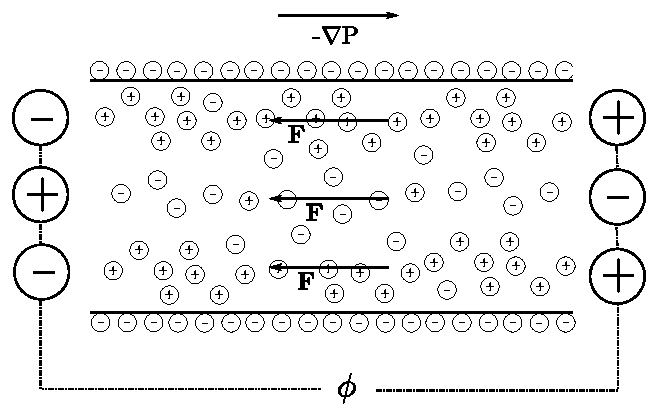
\includegraphics[width=0.7\textwidth]{fig/channel_electroviscous.pdf}
\end{center}
\caption[Example of an electroviscous system.]{Example of an
  electroviscous system. The fluid is driven by a pressure gradient,
  $\nabla \Prm$. The directions of the forces on the fluid are always
  opposite to the flow direction. The force originates from the
  potential difference, $\phi$, that builds up along the channel. The
  force is always opposite to the flow direction, thus slowing the
  flow down.}
\label{fig:et:ev}
\end{figure}


\subsection{Electroosmotic flow}\label{sec:et:electroosmosis}
Instead of driving the fluid flow through a pressure drop, a net
charged fluid may be driven by an external electric field. This may
be seen as the opposite case to that in section
\ref{sec:et:streaming_pot} where a current is induced by a pressure
drop.

The volumetric force on the fluid from the external field, $\E_{ext}$,
is given by

\begin{equation}
\F = \rhorm_e \E_{ext}
\end{equation}

where $\rho_e$ is the charge density. If the electric field is
constant (or at least has the same direction) everywhere, the sign of
the force is not in the same direction for a net charged positive area
of the fluid as for a net charged negative. Thus the fluid may be
either slowed down or sped up. This is a qualitative difference to
pressure driven situation and is illustrated in fig. \ref{fig:et:eo}.

\begin{figure}
\begin{center}
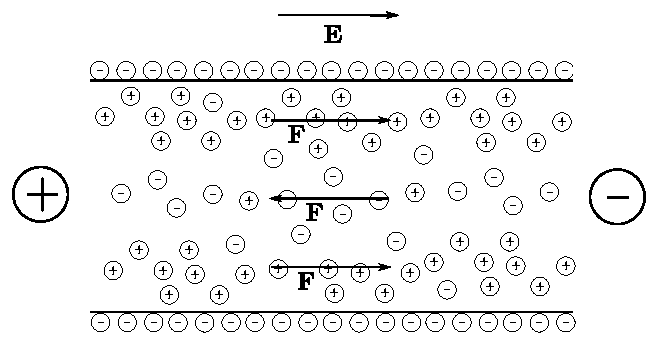
\includegraphics[width=0.7\textwidth]{fig/channel_electroosmosis.pdf}
\end{center}
\caption[Example of an electroosmotic system.]{Example of an
  electroosmotic system. The fluid is driven by an external electric
  field, $\E$. The directions of the forces on the fluid from the
  electric field are indicated with arrows. Note however that the
  fluid does not necessarily has to flow in the direction of the
  force, this due to viscous effects in the fluid. }
\label{fig:et:eo}
\end{figure}

The electroviscous effect is in the case of pure electroosmotic flow
usually neglected as the field due to the streaming potential is, in
most physical cases, small in comparison to the applied external
field. \cite{wang-poi}


%lite intro

%börja inte med allmän teorpmisk formulering

%sedan lite resultat, double layers

%pressure driven flows...
